% Options for packages loaded elsewhere
\PassOptionsToPackage{unicode}{hyperref}
\PassOptionsToPackage{hyphens}{url}
%
\documentclass[
]{article}
\usepackage{amsmath,amssymb}
\usepackage{lmodern}
\usepackage{iftex}
\ifPDFTeX
  \usepackage[T1]{fontenc}
  \usepackage[utf8]{inputenc}
  \usepackage{textcomp} % provide euro and other symbols
\else % if luatex or xetex
  \usepackage{unicode-math}
  \defaultfontfeatures{Scale=MatchLowercase}
  \defaultfontfeatures[\rmfamily]{Ligatures=TeX,Scale=1}
\fi
% Use upquote if available, for straight quotes in verbatim environments
\IfFileExists{upquote.sty}{\usepackage{upquote}}{}
\IfFileExists{microtype.sty}{% use microtype if available
  \usepackage[]{microtype}
  \UseMicrotypeSet[protrusion]{basicmath} % disable protrusion for tt fonts
}{}
\makeatletter
\@ifundefined{KOMAClassName}{% if non-KOMA class
  \IfFileExists{parskip.sty}{%
    \usepackage{parskip}
  }{% else
    \setlength{\parindent}{0pt}
    \setlength{\parskip}{6pt plus 2pt minus 1pt}}
}{% if KOMA class
  \KOMAoptions{parskip=half}}
\makeatother
\usepackage{xcolor}
\usepackage[margin=1in]{geometry}
\usepackage{color}
\usepackage{fancyvrb}
\newcommand{\VerbBar}{|}
\newcommand{\VERB}{\Verb[commandchars=\\\{\}]}
\DefineVerbatimEnvironment{Highlighting}{Verbatim}{commandchars=\\\{\}}
% Add ',fontsize=\small' for more characters per line
\usepackage{framed}
\definecolor{shadecolor}{RGB}{248,248,248}
\newenvironment{Shaded}{\begin{snugshade}}{\end{snugshade}}
\newcommand{\AlertTok}[1]{\textcolor[rgb]{0.94,0.16,0.16}{#1}}
\newcommand{\AnnotationTok}[1]{\textcolor[rgb]{0.56,0.35,0.01}{\textbf{\textit{#1}}}}
\newcommand{\AttributeTok}[1]{\textcolor[rgb]{0.77,0.63,0.00}{#1}}
\newcommand{\BaseNTok}[1]{\textcolor[rgb]{0.00,0.00,0.81}{#1}}
\newcommand{\BuiltInTok}[1]{#1}
\newcommand{\CharTok}[1]{\textcolor[rgb]{0.31,0.60,0.02}{#1}}
\newcommand{\CommentTok}[1]{\textcolor[rgb]{0.56,0.35,0.01}{\textit{#1}}}
\newcommand{\CommentVarTok}[1]{\textcolor[rgb]{0.56,0.35,0.01}{\textbf{\textit{#1}}}}
\newcommand{\ConstantTok}[1]{\textcolor[rgb]{0.00,0.00,0.00}{#1}}
\newcommand{\ControlFlowTok}[1]{\textcolor[rgb]{0.13,0.29,0.53}{\textbf{#1}}}
\newcommand{\DataTypeTok}[1]{\textcolor[rgb]{0.13,0.29,0.53}{#1}}
\newcommand{\DecValTok}[1]{\textcolor[rgb]{0.00,0.00,0.81}{#1}}
\newcommand{\DocumentationTok}[1]{\textcolor[rgb]{0.56,0.35,0.01}{\textbf{\textit{#1}}}}
\newcommand{\ErrorTok}[1]{\textcolor[rgb]{0.64,0.00,0.00}{\textbf{#1}}}
\newcommand{\ExtensionTok}[1]{#1}
\newcommand{\FloatTok}[1]{\textcolor[rgb]{0.00,0.00,0.81}{#1}}
\newcommand{\FunctionTok}[1]{\textcolor[rgb]{0.00,0.00,0.00}{#1}}
\newcommand{\ImportTok}[1]{#1}
\newcommand{\InformationTok}[1]{\textcolor[rgb]{0.56,0.35,0.01}{\textbf{\textit{#1}}}}
\newcommand{\KeywordTok}[1]{\textcolor[rgb]{0.13,0.29,0.53}{\textbf{#1}}}
\newcommand{\NormalTok}[1]{#1}
\newcommand{\OperatorTok}[1]{\textcolor[rgb]{0.81,0.36,0.00}{\textbf{#1}}}
\newcommand{\OtherTok}[1]{\textcolor[rgb]{0.56,0.35,0.01}{#1}}
\newcommand{\PreprocessorTok}[1]{\textcolor[rgb]{0.56,0.35,0.01}{\textit{#1}}}
\newcommand{\RegionMarkerTok}[1]{#1}
\newcommand{\SpecialCharTok}[1]{\textcolor[rgb]{0.00,0.00,0.00}{#1}}
\newcommand{\SpecialStringTok}[1]{\textcolor[rgb]{0.31,0.60,0.02}{#1}}
\newcommand{\StringTok}[1]{\textcolor[rgb]{0.31,0.60,0.02}{#1}}
\newcommand{\VariableTok}[1]{\textcolor[rgb]{0.00,0.00,0.00}{#1}}
\newcommand{\VerbatimStringTok}[1]{\textcolor[rgb]{0.31,0.60,0.02}{#1}}
\newcommand{\WarningTok}[1]{\textcolor[rgb]{0.56,0.35,0.01}{\textbf{\textit{#1}}}}
\usepackage{longtable,booktabs,array}
\usepackage{calc} % for calculating minipage widths
% Correct order of tables after \paragraph or \subparagraph
\usepackage{etoolbox}
\makeatletter
\patchcmd\longtable{\par}{\if@noskipsec\mbox{}\fi\par}{}{}
\makeatother
% Allow footnotes in longtable head/foot
\IfFileExists{footnotehyper.sty}{\usepackage{footnotehyper}}{\usepackage{footnote}}
\makesavenoteenv{longtable}
\usepackage{graphicx}
\makeatletter
\def\maxwidth{\ifdim\Gin@nat@width>\linewidth\linewidth\else\Gin@nat@width\fi}
\def\maxheight{\ifdim\Gin@nat@height>\textheight\textheight\else\Gin@nat@height\fi}
\makeatother
% Scale images if necessary, so that they will not overflow the page
% margins by default, and it is still possible to overwrite the defaults
% using explicit options in \includegraphics[width, height, ...]{}
\setkeys{Gin}{width=\maxwidth,height=\maxheight,keepaspectratio}
% Set default figure placement to htbp
\makeatletter
\def\fps@figure{htbp}
\makeatother
\setlength{\emergencystretch}{3em} % prevent overfull lines
\providecommand{\tightlist}{%
  \setlength{\itemsep}{0pt}\setlength{\parskip}{0pt}}
\setcounter{secnumdepth}{-\maxdimen} % remove section numbering
\ifLuaTeX
  \usepackage{selnolig}  % disable illegal ligatures
\fi
\IfFileExists{bookmark.sty}{\usepackage{bookmark}}{\usepackage{hyperref}}
\IfFileExists{xurl.sty}{\usepackage{xurl}}{} % add URL line breaks if available
\urlstyle{same} % disable monospaced font for URLs
\hypersetup{
  pdftitle={PSTAT 126 Project Step 1},
  pdfauthor={Angel Abdulnour, Andrew Hansen, Sammy Suliman},
  hidelinks,
  pdfcreator={LaTeX via pandoc}}

\title{PSTAT 126 Project Step 1}
\author{Angel Abdulnour, Andrew Hansen, Sammy Suliman}
\date{2023-04-29}

\begin{document}
\maketitle

\begin{Shaded}
\begin{Highlighting}[]
\NormalTok{performance }\OtherTok{\textless{}{-}} \FunctionTok{read.csv}\NormalTok{(}\StringTok{"C:/Users/filto/Desktop/PSTAT\_126/project2/student/student{-}por.csv"}\NormalTok{, }\AttributeTok{header=}\ConstantTok{TRUE}\NormalTok{, }\AttributeTok{stringsAsFactors=}\ConstantTok{FALSE}\NormalTok{, }\AttributeTok{sep=}\StringTok{\textquotesingle{};\textquotesingle{}}\NormalTok{)}
\CommentTok{\#performance}
\end{Highlighting}
\end{Shaded}

Our dataset is the student performance dataset, measuring the
association between student's grades and a list of 33 numeric and
categorical variables.

Let's get a summary of our data including number of rows, number of
columns, and how many numeric and character variables there are.

\begin{Shaded}
\begin{Highlighting}[]
\FunctionTok{skim}\NormalTok{(performance)}
\end{Highlighting}
\end{Shaded}

\begin{longtable}[]{@{}ll@{}}
\caption{Data summary}\tabularnewline
\toprule()
\endhead
Name & performance \\
Number of rows & 649 \\
Number of columns & 33 \\
\_\_\_\_\_\_\_\_\_\_\_\_\_\_\_\_\_\_\_\_\_\_\_ & \\
Column type frequency: & \\
character & 17 \\
numeric & 16 \\
\_\_\_\_\_\_\_\_\_\_\_\_\_\_\_\_\_\_\_\_\_\_\_\_ & \\
Group variables & None \\
\bottomrule()
\end{longtable}

\textbf{Variable type: character}

\begin{longtable}[]{@{}
  >{\raggedright\arraybackslash}p{(\columnwidth - 14\tabcolsep) * \real{0.1944}}
  >{\raggedleft\arraybackslash}p{(\columnwidth - 14\tabcolsep) * \real{0.1389}}
  >{\raggedleft\arraybackslash}p{(\columnwidth - 14\tabcolsep) * \real{0.1944}}
  >{\raggedleft\arraybackslash}p{(\columnwidth - 14\tabcolsep) * \real{0.0556}}
  >{\raggedleft\arraybackslash}p{(\columnwidth - 14\tabcolsep) * \real{0.0556}}
  >{\raggedleft\arraybackslash}p{(\columnwidth - 14\tabcolsep) * \real{0.0833}}
  >{\raggedleft\arraybackslash}p{(\columnwidth - 14\tabcolsep) * \real{0.1250}}
  >{\raggedleft\arraybackslash}p{(\columnwidth - 14\tabcolsep) * \real{0.1528}}@{}}
\toprule()
\begin{minipage}[b]{\linewidth}\raggedright
skim\_variable
\end{minipage} & \begin{minipage}[b]{\linewidth}\raggedleft
n\_missing
\end{minipage} & \begin{minipage}[b]{\linewidth}\raggedleft
complete\_rate
\end{minipage} & \begin{minipage}[b]{\linewidth}\raggedleft
min
\end{minipage} & \begin{minipage}[b]{\linewidth}\raggedleft
max
\end{minipage} & \begin{minipage}[b]{\linewidth}\raggedleft
empty
\end{minipage} & \begin{minipage}[b]{\linewidth}\raggedleft
n\_unique
\end{minipage} & \begin{minipage}[b]{\linewidth}\raggedleft
whitespace
\end{minipage} \\
\midrule()
\endhead
school & 0 & 1 & 2 & 2 & 0 & 2 & 0 \\
sex & 0 & 1 & 1 & 1 & 0 & 2 & 0 \\
address & 0 & 1 & 1 & 1 & 0 & 2 & 0 \\
famsize & 0 & 1 & 3 & 3 & 0 & 2 & 0 \\
Pstatus & 0 & 1 & 1 & 1 & 0 & 2 & 0 \\
Mjob & 0 & 1 & 5 & 8 & 0 & 5 & 0 \\
Fjob & 0 & 1 & 5 & 8 & 0 & 5 & 0 \\
reason & 0 & 1 & 4 & 10 & 0 & 4 & 0 \\
guardian & 0 & 1 & 5 & 6 & 0 & 3 & 0 \\
schoolsup & 0 & 1 & 2 & 3 & 0 & 2 & 0 \\
famsup & 0 & 1 & 2 & 3 & 0 & 2 & 0 \\
paid & 0 & 1 & 2 & 3 & 0 & 2 & 0 \\
activities & 0 & 1 & 2 & 3 & 0 & 2 & 0 \\
nursery & 0 & 1 & 2 & 3 & 0 & 2 & 0 \\
higher & 0 & 1 & 2 & 3 & 0 & 2 & 0 \\
internet & 0 & 1 & 2 & 3 & 0 & 2 & 0 \\
romantic & 0 & 1 & 2 & 3 & 0 & 2 & 0 \\
\bottomrule()
\end{longtable}

\textbf{Variable type: numeric}

\begin{longtable}[]{@{}
  >{\raggedright\arraybackslash}p{(\columnwidth - 20\tabcolsep) * \real{0.1273}}
  >{\raggedleft\arraybackslash}p{(\columnwidth - 20\tabcolsep) * \real{0.0909}}
  >{\raggedleft\arraybackslash}p{(\columnwidth - 20\tabcolsep) * \real{0.1273}}
  >{\raggedleft\arraybackslash}p{(\columnwidth - 20\tabcolsep) * \real{0.0545}}
  >{\raggedleft\arraybackslash}p{(\columnwidth - 20\tabcolsep) * \real{0.0455}}
  >{\raggedleft\arraybackslash}p{(\columnwidth - 20\tabcolsep) * \real{0.0273}}
  >{\raggedleft\arraybackslash}p{(\columnwidth - 20\tabcolsep) * \real{0.0364}}
  >{\raggedleft\arraybackslash}p{(\columnwidth - 20\tabcolsep) * \real{0.0364}}
  >{\raggedleft\arraybackslash}p{(\columnwidth - 20\tabcolsep) * \real{0.0364}}
  >{\raggedleft\arraybackslash}p{(\columnwidth - 20\tabcolsep) * \real{0.0455}}
  >{\raggedright\arraybackslash}p{(\columnwidth - 20\tabcolsep) * \real{0.3727}}@{}}
\toprule()
\begin{minipage}[b]{\linewidth}\raggedright
skim\_variable
\end{minipage} & \begin{minipage}[b]{\linewidth}\raggedleft
n\_missing
\end{minipage} & \begin{minipage}[b]{\linewidth}\raggedleft
complete\_rate
\end{minipage} & \begin{minipage}[b]{\linewidth}\raggedleft
mean
\end{minipage} & \begin{minipage}[b]{\linewidth}\raggedleft
sd
\end{minipage} & \begin{minipage}[b]{\linewidth}\raggedleft
p0
\end{minipage} & \begin{minipage}[b]{\linewidth}\raggedleft
p25
\end{minipage} & \begin{minipage}[b]{\linewidth}\raggedleft
p50
\end{minipage} & \begin{minipage}[b]{\linewidth}\raggedleft
p75
\end{minipage} & \begin{minipage}[b]{\linewidth}\raggedleft
p100
\end{minipage} & \begin{minipage}[b]{\linewidth}\raggedright
hist
\end{minipage} \\
\midrule()
\endhead
age & 0 & 1 & 16.74 & 1.22 & 15 & 16 & 17 & 18 & 22 & ▇▅▅▁▁ \\
Medu & 0 & 1 & 2.51 & 1.13 & 0 & 2 & 2 & 4 & 4 & ▁▆▇▆▇ \\
Fedu & 0 & 1 & 2.31 & 1.10 & 0 & 1 & 2 & 3 & 4 & ▁▆▇▅▅ \\
traveltime & 0 & 1 & 1.57 & 0.75 & 1 & 1 & 1 & 2 & 4 & ▇▅▁▁▁ \\
studytime & 0 & 1 & 1.93 & 0.83 & 1 & 1 & 2 & 2 & 4 & ▆▇▁▂▁ \\
failures & 0 & 1 & 0.22 & 0.59 & 0 & 0 & 0 & 0 & 3 & ▇▁▁▁▁ \\
famrel & 0 & 1 & 3.93 & 0.96 & 1 & 4 & 4 & 5 & 5 & ▁▁▂▇▅ \\
freetime & 0 & 1 & 3.18 & 1.05 & 1 & 3 & 3 & 4 & 5 & ▂▃▇▆▂ \\
goout & 0 & 1 & 3.18 & 1.18 & 1 & 2 & 3 & 4 & 5 & ▂▆▇▆▅ \\
Dalc & 0 & 1 & 1.50 & 0.92 & 1 & 1 & 1 & 2 & 5 & ▇▂▁▁▁ \\
Walc & 0 & 1 & 2.28 & 1.28 & 1 & 1 & 2 & 3 & 5 & ▇▅▃▃▂ \\
health & 0 & 1 & 3.54 & 1.45 & 1 & 2 & 4 & 5 & 5 & ▃▂▃▃▇ \\
absences & 0 & 1 & 3.66 & 4.64 & 0 & 0 & 2 & 6 & 32 & ▇▂▁▁▁ \\
G1 & 0 & 1 & 11.40 & 2.75 & 0 & 10 & 11 & 13 & 19 & ▁▂▇▇▁ \\
G2 & 0 & 1 & 11.57 & 2.91 & 0 & 10 & 11 & 13 & 19 & ▁▁▇▇▂ \\
G3 & 0 & 1 & 11.91 & 3.23 & 0 & 10 & 12 & 14 & 19 & ▁▁▇▇▂ \\
\bottomrule()
\end{longtable}

Our dataset consists of For the purposes of our regresWe want to test
the normality of our response variable. We will do this through a
statistical test (Shapiro-Wilk) and ply creating QQ plots of the
response

\begin{Shaded}
\begin{Highlighting}[]
\CommentTok{\# tests the normality of the G3 response variable}
\FunctionTok{shapiro.test}\NormalTok{(performance}\SpecialCharTok{$}\NormalTok{G3)}
\end{Highlighting}
\end{Shaded}

\begin{verbatim}
## 
##  Shapiro-Wilk normality test
## 
## data:  performance$G3
## W = 0.92598, p-value < 2.2e-16
\end{verbatim}

Since the Shapiro-Wilk test results in P-Values less than 0.05, we
conclude that G3, our response varible, is not normally distributed.

Now that we identified that our response is not normal, let's check all
of our numeric independent variables for normality

\begin{Shaded}
\begin{Highlighting}[]
\CommentTok{\#gives qq plot of G3 response variable}
\FunctionTok{qqnorm}\NormalTok{(performance}\SpecialCharTok{$}\NormalTok{G3)}
\FunctionTok{qqline}\NormalTok{(performance}\SpecialCharTok{$}\NormalTok{G3)}
\end{Highlighting}
\end{Shaded}

\includegraphics{pstat_126_project_Week1_files/figure-latex/unnamed-chunk-4-1.pdf}

Numeric performace is a subset of Performance which focuses solely on
the numeric data. With it we can create Histogram and qq plots of the 16
numeric variables

\begin{Shaded}
\begin{Highlighting}[]
\NormalTok{numeric\_performance }\OtherTok{\textless{}{-}}\NormalTok{ performance }\SpecialCharTok{\%\textgreater{}\%} \FunctionTok{select\_if}\NormalTok{(is.numeric)}
\CommentTok{\#x\textless{}{-}(numeric\_performance$age)}
\CommentTok{\#y\textless{}{-}dnorm(numeric\_performance$age)}
\CommentTok{\#plot(x,y)}
\CommentTok{\#barplot(numeric\_performance$age)}
\CommentTok{\#qqnorm(numeric\_performance$age)}

\ControlFlowTok{for}\NormalTok{ (i }\ControlFlowTok{in} \DecValTok{1}\SpecialCharTok{:}\FunctionTok{ncol}\NormalTok{(numeric\_performance))\{}
\FunctionTok{par}\NormalTok{(}\AttributeTok{mfrow=}\FunctionTok{c}\NormalTok{(}\DecValTok{1}\NormalTok{,}\DecValTok{2}\NormalTok{))}
\CommentTok{\#x\textless{}{-}(numeric\_performance[,1])}
\CommentTok{\#y\textless{}{-}dnorm(numeric\_performance[,1])}
\CommentTok{\#plot(x,y)}
\FunctionTok{hist}\NormalTok{(numeric\_performance[,i])}
\CommentTok{\#barplot(numeric\_performance[,1])}


\FunctionTok{qqnorm}\NormalTok{(numeric\_performance[,i])}
\FunctionTok{qqline}\NormalTok{(numeric\_performance[,i])}
\NormalTok{\}}
\end{Highlighting}
\end{Shaded}

\includegraphics{pstat_126_project_Week1_files/figure-latex/unnamed-chunk-5-1.pdf}
\includegraphics{pstat_126_project_Week1_files/figure-latex/unnamed-chunk-5-2.pdf}
\includegraphics{pstat_126_project_Week1_files/figure-latex/unnamed-chunk-5-3.pdf}
\includegraphics{pstat_126_project_Week1_files/figure-latex/unnamed-chunk-5-4.pdf}
\includegraphics{pstat_126_project_Week1_files/figure-latex/unnamed-chunk-5-5.pdf}
\includegraphics{pstat_126_project_Week1_files/figure-latex/unnamed-chunk-5-6.pdf}
\includegraphics{pstat_126_project_Week1_files/figure-latex/unnamed-chunk-5-7.pdf}
\includegraphics{pstat_126_project_Week1_files/figure-latex/unnamed-chunk-5-8.pdf}
\includegraphics{pstat_126_project_Week1_files/figure-latex/unnamed-chunk-5-9.pdf}
\includegraphics{pstat_126_project_Week1_files/figure-latex/unnamed-chunk-5-10.pdf}
\includegraphics{pstat_126_project_Week1_files/figure-latex/unnamed-chunk-5-11.pdf}
\includegraphics{pstat_126_project_Week1_files/figure-latex/unnamed-chunk-5-12.pdf}
\includegraphics{pstat_126_project_Week1_files/figure-latex/unnamed-chunk-5-13.pdf}
\includegraphics{pstat_126_project_Week1_files/figure-latex/unnamed-chunk-5-14.pdf}
\includegraphics{pstat_126_project_Week1_files/figure-latex/unnamed-chunk-5-15.pdf}
\includegraphics{pstat_126_project_Week1_files/figure-latex/unnamed-chunk-5-16.pdf}
Looking at the QQ plots and histograms above one can clearly tell they
are not normally distributed. However, just to make sure we ran the
shapiro test and we can see that all the variables have a p-value less
than 0.05 meaning none of them are normally distributed.

\begin{Shaded}
\begin{Highlighting}[]
\NormalTok{loopShapiro }\OtherTok{\textless{}{-}} \FunctionTok{list}\NormalTok{()}
\ControlFlowTok{for}\NormalTok{ (i }\ControlFlowTok{in} \DecValTok{1}\SpecialCharTok{:}\FunctionTok{ncol}\NormalTok{(numeric\_performance))\{}
\NormalTok{loopShapiro[i] }\OtherTok{\textless{}{-}} \FunctionTok{shapiro.test}\NormalTok{(numeric\_performance[,i])}\SpecialCharTok{$}\NormalTok{p.value}

\NormalTok{\}}
\NormalTok{loopShapiro}
\end{Highlighting}
\end{Shaded}

\begin{verbatim}
## [[1]]
## [1] 1.519202e-18
## 
## [[2]]
## [1] 7.899347e-23
## 
## [[3]]
## [1] 2.147426e-22
## 
## [[4]]
## [1] 2.503463e-31
## 
## [[5]]
## [1] 5.22241e-26
## 
## [[6]]
## [1] 3.852717e-41
## 
## [[7]]
## [1] 1.82721e-26
## 
## [[8]]
## [1] 3.78657e-19
## 
## [[9]]
## [1] 5.243927e-19
## 
## [[10]]
## [1] 4.417427e-36
## 
## [[11]]
## [1] 1.219194e-24
## 
## [[12]]
## [1] 3.278214e-25
## 
## [[13]]
## [1] 4.522443e-29
## 
## [[14]]
## [1] 4.933521e-06
## 
## [[15]]
## [1] 5.583292e-12
## 
## [[16]]
## [1] 2.415986e-17
\end{verbatim}

Seeing that none of the variables are normal we attempt to normalize
them by using a few different methods. The first method is a scaling
method where we base it around the mean. Below we create a data frame
that scales numer\_performance and provide a summary of its data.

\begin{Shaded}
\begin{Highlighting}[]
\CommentTok{\#normalize method 1}

\CommentTok{\#plot(x = numeric\_performance$traveltime, y = dnorm(numeric\_performance$traveltime), type="l", bty="n")}
\NormalTok{scaled\_numeric\_performance1 }\OtherTok{\textless{}{-}} \FunctionTok{as.data.frame}\NormalTok{(}\FunctionTok{scale}\NormalTok{(numeric\_performance))}
\FunctionTok{summary}\NormalTok{(scaled\_numeric\_performance1)}
\end{Highlighting}
\end{Shaded}

\begin{verbatim}
##       age              Medu              Fedu           traveltime     
##  Min.   :-1.432   Min.   :-2.2164   Min.   :-2.0971   Min.   :-0.7594  
##  1st Qu.:-0.611   1st Qu.:-0.4536   1st Qu.:-1.1879   1st Qu.:-0.7594  
##  Median : 0.210   Median :-0.4536   Median :-0.2788   Median :-0.7594  
##  Mean   : 0.000   Mean   : 0.0000   Mean   : 0.0000   Mean   : 0.0000  
##  3rd Qu.: 1.031   3rd Qu.: 1.3092   3rd Qu.: 0.6304   3rd Qu.: 0.5763  
##  Max.   : 4.315   Max.   : 1.3092   Max.   : 1.5395   Max.   : 3.2477  
##    studytime           failures          famrel            freetime      
##  Min.   :-1.12194   Min.   :-0.374   Min.   :-3.06645   Min.   :-2.0743  
##  1st Qu.:-1.12194   1st Qu.:-0.374   1st Qu.: 0.07255   1st Qu.:-0.1715  
##  Median : 0.08359   Median :-0.374   Median : 0.07255   Median :-0.1715  
##  Mean   : 0.00000   Mean   : 0.000   Mean   : 0.00000   Mean   : 0.0000  
##  3rd Qu.: 0.08359   3rd Qu.:-0.374   3rd Qu.: 1.11889   3rd Qu.: 0.7799  
##  Max.   : 2.49465   Max.   : 4.683   Max.   : 1.11889   Max.   : 1.7313  
##      goout              Dalc              Walc             health       
##  Min.   :-1.8583   Min.   :-0.5431   Min.   :-0.9969   Min.   :-1.7536  
##  1st Qu.:-1.0078   1st Qu.:-0.5431   1st Qu.:-0.9969   1st Qu.:-1.0622  
##  Median :-0.1573   Median :-0.5431   Median :-0.2183   Median : 0.3207  
##  Mean   : 0.0000   Mean   : 0.0000   Mean   : 0.0000   Mean   : 0.0000  
##  3rd Qu.: 0.6933   3rd Qu.: 0.5381   3rd Qu.: 0.5602   3rd Qu.: 1.0121  
##  Max.   : 1.5438   Max.   : 3.7820   Max.   : 2.1174   Max.   : 1.0121  
##     absences             G1                G2                G3          
##  Min.   :-0.7886   Min.   :-4.1523   Min.   :-3.9710   Min.   :-3.68532  
##  1st Qu.:-0.7886   1st Qu.:-0.5096   1st Qu.:-0.5389   1st Qu.:-0.58998  
##  Median :-0.3576   Median :-0.1454   Median :-0.1957   Median : 0.02909  
##  Mean   : 0.0000   Mean   : 0.0000   Mean   : 0.0000   Mean   : 0.00000  
##  3rd Qu.: 0.5043   3rd Qu.: 0.5832   3rd Qu.: 0.4908   3rd Qu.: 0.64816  
##  Max.   : 6.1069   Max.   : 2.7687   Max.   : 2.5500   Max.   : 2.19584
\end{verbatim}

Next we create histograms and QQ plots of scaled\_numeric\_performance1.
However many of the variables clearly show distributions that are not
normal. the only ones that appear normal are G1, G2, and G3.

\begin{Shaded}
\begin{Highlighting}[]
\ControlFlowTok{for}\NormalTok{ (i }\ControlFlowTok{in} \DecValTok{1}\SpecialCharTok{:}\FunctionTok{ncol}\NormalTok{(scaled\_numeric\_performance1))\{}
  \FunctionTok{par}\NormalTok{(}\AttributeTok{mfrow=}\FunctionTok{c}\NormalTok{(}\DecValTok{1}\NormalTok{,}\DecValTok{2}\NormalTok{))}
  \FunctionTok{hist}\NormalTok{(scaled\_numeric\_performance1[,i])}
  \FunctionTok{qqnorm}\NormalTok{(scaled\_numeric\_performance1[,i])}
  \FunctionTok{qqline}\NormalTok{(scaled\_numeric\_performance1[,i])}
\NormalTok{\}}
\end{Highlighting}
\end{Shaded}

\includegraphics{pstat_126_project_Week1_files/figure-latex/unnamed-chunk-8-1.pdf}
\includegraphics{pstat_126_project_Week1_files/figure-latex/unnamed-chunk-8-2.pdf}
\includegraphics{pstat_126_project_Week1_files/figure-latex/unnamed-chunk-8-3.pdf}
\includegraphics{pstat_126_project_Week1_files/figure-latex/unnamed-chunk-8-4.pdf}
\includegraphics{pstat_126_project_Week1_files/figure-latex/unnamed-chunk-8-5.pdf}
\includegraphics{pstat_126_project_Week1_files/figure-latex/unnamed-chunk-8-6.pdf}
\includegraphics{pstat_126_project_Week1_files/figure-latex/unnamed-chunk-8-7.pdf}
\includegraphics{pstat_126_project_Week1_files/figure-latex/unnamed-chunk-8-8.pdf}
\includegraphics{pstat_126_project_Week1_files/figure-latex/unnamed-chunk-8-9.pdf}
\includegraphics{pstat_126_project_Week1_files/figure-latex/unnamed-chunk-8-10.pdf}
\includegraphics{pstat_126_project_Week1_files/figure-latex/unnamed-chunk-8-11.pdf}
\includegraphics{pstat_126_project_Week1_files/figure-latex/unnamed-chunk-8-12.pdf}
\includegraphics{pstat_126_project_Week1_files/figure-latex/unnamed-chunk-8-13.pdf}
\includegraphics{pstat_126_project_Week1_files/figure-latex/unnamed-chunk-8-14.pdf}
\includegraphics{pstat_126_project_Week1_files/figure-latex/unnamed-chunk-8-15.pdf}
\includegraphics{pstat_126_project_Week1_files/figure-latex/unnamed-chunk-8-16.pdf}

\begin{Shaded}
\begin{Highlighting}[]
\CommentTok{\#hist(scaled\_numeric\_performance$age)}
\CommentTok{\#plot(x = scaled\_numeric\_performance$age, y = dnorm(scaled\_numeric\_performance$age))}
\CommentTok{\#norm\_scaled\_numeric\_performance1 \textless{}{-} predict(scaled\_numeric\_performance1, as.data.frame(numeric\_performance))}
\CommentTok{\#hist(norm\_scaled\_numeric\_performance2$goout)}
\CommentTok{\#plot(x = norm\_scaled\_numeric\_performance2$age, y = dnorm(norm\_scaled\_numeric\_performance2$age))}
\end{Highlighting}
\end{Shaded}

To make sure our information is accurate we run Shpairo tests on
scaled\_numeric\_performance1 and find that all, including G1, G2, G3,
are not normal since their P-Values are all under 0.05.

\begin{Shaded}
\begin{Highlighting}[]
\NormalTok{scaledLoopShapiro1 }\OtherTok{\textless{}{-}} \FunctionTok{list}\NormalTok{()}
\ControlFlowTok{for}\NormalTok{ (i }\ControlFlowTok{in} \DecValTok{1}\SpecialCharTok{:}\FunctionTok{ncol}\NormalTok{(scaled\_numeric\_performance1))\{}
\NormalTok{scaledLoopShapiro1[i] }\OtherTok{\textless{}{-}} \FunctionTok{shapiro.test}\NormalTok{(scaled\_numeric\_performance1[,i])}\SpecialCharTok{$}\NormalTok{p.value}

\NormalTok{\}}
\NormalTok{scaledLoopShapiro1}
\end{Highlighting}
\end{Shaded}

\begin{verbatim}
## [[1]]
## [1] 1.519202e-18
## 
## [[2]]
## [1] 7.899347e-23
## 
## [[3]]
## [1] 2.147426e-22
## 
## [[4]]
## [1] 2.503463e-31
## 
## [[5]]
## [1] 5.22241e-26
## 
## [[6]]
## [1] 3.852717e-41
## 
## [[7]]
## [1] 1.82721e-26
## 
## [[8]]
## [1] 3.78657e-19
## 
## [[9]]
## [1] 5.243927e-19
## 
## [[10]]
## [1] 4.417427e-36
## 
## [[11]]
## [1] 1.219194e-24
## 
## [[12]]
## [1] 3.278214e-25
## 
## [[13]]
## [1] 4.522443e-29
## 
## [[14]]
## [1] 4.933521e-06
## 
## [[15]]
## [1] 5.583292e-12
## 
## [[16]]
## [1] 2.415986e-17
\end{verbatim}

The second scaling method that we use is one were we set a range from 0
to 1 and cram the data into that range. to do this we created another
data set called scaled\_numeric\_performance2 to store that scaled
information. Below is a summary of the scaled data

\begin{Shaded}
\begin{Highlighting}[]
\CommentTok{\#normalize method 2}
\NormalTok{scaled\_numeric\_performance2 }\OtherTok{\textless{}{-}} \FunctionTok{preProcess}\NormalTok{(}\FunctionTok{as.data.frame}\NormalTok{(numeric\_performance), }\AttributeTok{method=}\FunctionTok{c}\NormalTok{(}\StringTok{\textquotesingle{}range\textquotesingle{}}\NormalTok{))}
\NormalTok{norm\_scaled\_numeric\_performance2 }\OtherTok{\textless{}{-}} \FunctionTok{predict}\NormalTok{(scaled\_numeric\_performance2, }\FunctionTok{as.data.frame}\NormalTok{(numeric\_performance))}
\FunctionTok{summary}\NormalTok{(norm\_scaled\_numeric\_performance2)}
\end{Highlighting}
\end{Shaded}

\begin{verbatim}
##       age              Medu             Fedu          traveltime    
##  Min.   :0.0000   Min.   :0.0000   Min.   :0.0000   Min.   :0.0000  
##  1st Qu.:0.1429   1st Qu.:0.5000   1st Qu.:0.2500   1st Qu.:0.0000  
##  Median :0.2857   Median :0.5000   Median :0.5000   Median :0.0000  
##  Mean   :0.2492   Mean   :0.6287   Mean   :0.5767   Mean   :0.1895  
##  3rd Qu.:0.4286   3rd Qu.:1.0000   3rd Qu.:0.7500   3rd Qu.:0.3333  
##  Max.   :1.0000   Max.   :1.0000   Max.   :1.0000   Max.   :1.0000  
##    studytime         failures           famrel          freetime     
##  Min.   :0.0000   Min.   :0.00000   Min.   :0.0000   Min.   :0.0000  
##  1st Qu.:0.0000   1st Qu.:0.00000   1st Qu.:0.7500   1st Qu.:0.5000  
##  Median :0.3333   Median :0.00000   Median :0.7500   Median :0.5000  
##  Mean   :0.3102   Mean   :0.07396   Mean   :0.7327   Mean   :0.5451  
##  3rd Qu.:0.3333   3rd Qu.:0.00000   3rd Qu.:1.0000   3rd Qu.:0.7500  
##  Max.   :1.0000   Max.   :1.00000   Max.   :1.0000   Max.   :1.0000  
##      goout             Dalc             Walc            health      
##  Min.   :0.0000   Min.   :0.0000   Min.   :0.0000   Min.   :0.0000  
##  1st Qu.:0.2500   1st Qu.:0.0000   1st Qu.:0.0000   1st Qu.:0.2500  
##  Median :0.5000   Median :0.0000   Median :0.2500   Median :0.7500  
##  Mean   :0.5462   Mean   :0.1256   Mean   :0.3201   Mean   :0.6341  
##  3rd Qu.:0.7500   3rd Qu.:0.2500   3rd Qu.:0.5000   3rd Qu.:1.0000  
##  Max.   :1.0000   Max.   :1.0000   Max.   :1.0000   Max.   :1.0000  
##     absences            G1               G2               G3        
##  Min.   :0.0000   Min.   :0.0000   Min.   :0.0000   Min.   :0.0000  
##  1st Qu.:0.0000   1st Qu.:0.5263   1st Qu.:0.5263   1st Qu.:0.5263  
##  Median :0.0625   Median :0.5789   Median :0.5789   Median :0.6316  
##  Mean   :0.1144   Mean   :0.6000   Mean   :0.6090   Mean   :0.6266  
##  3rd Qu.:0.1875   3rd Qu.:0.6842   3rd Qu.:0.6842   3rd Qu.:0.7368  
##  Max.   :1.0000   Max.   :1.0000   Max.   :1.0000   Max.   :1.0000
\end{verbatim}

Using the data from norm\_scaled\_numeric\_performance2 we create
histograms and QQ plots to try to gauge the normality. Once again we see
the G1, G2, and G3 variables be normal but not the others.

\begin{Shaded}
\begin{Highlighting}[]
\ControlFlowTok{for}\NormalTok{ (i }\ControlFlowTok{in} \DecValTok{1}\SpecialCharTok{:}\FunctionTok{ncol}\NormalTok{(norm\_scaled\_numeric\_performance2))\{}
  \FunctionTok{par}\NormalTok{(}\AttributeTok{mfrow=}\FunctionTok{c}\NormalTok{(}\DecValTok{1}\NormalTok{,}\DecValTok{2}\NormalTok{))}
  \FunctionTok{hist}\NormalTok{(norm\_scaled\_numeric\_performance2[,i])}
  \FunctionTok{qqnorm}\NormalTok{(norm\_scaled\_numeric\_performance2[,i])}
  \FunctionTok{qqline}\NormalTok{(norm\_scaled\_numeric\_performance2[,i])}
\NormalTok{\}}
\end{Highlighting}
\end{Shaded}

\includegraphics{pstat_126_project_Week1_files/figure-latex/unnamed-chunk-11-1.pdf}
\includegraphics{pstat_126_project_Week1_files/figure-latex/unnamed-chunk-11-2.pdf}
\includegraphics{pstat_126_project_Week1_files/figure-latex/unnamed-chunk-11-3.pdf}
\includegraphics{pstat_126_project_Week1_files/figure-latex/unnamed-chunk-11-4.pdf}
\includegraphics{pstat_126_project_Week1_files/figure-latex/unnamed-chunk-11-5.pdf}
\includegraphics{pstat_126_project_Week1_files/figure-latex/unnamed-chunk-11-6.pdf}
\includegraphics{pstat_126_project_Week1_files/figure-latex/unnamed-chunk-11-7.pdf}
\includegraphics{pstat_126_project_Week1_files/figure-latex/unnamed-chunk-11-8.pdf}
\includegraphics{pstat_126_project_Week1_files/figure-latex/unnamed-chunk-11-9.pdf}
\includegraphics{pstat_126_project_Week1_files/figure-latex/unnamed-chunk-11-10.pdf}
\includegraphics{pstat_126_project_Week1_files/figure-latex/unnamed-chunk-11-11.pdf}
\includegraphics{pstat_126_project_Week1_files/figure-latex/unnamed-chunk-11-12.pdf}
\includegraphics{pstat_126_project_Week1_files/figure-latex/unnamed-chunk-11-13.pdf}
\includegraphics{pstat_126_project_Week1_files/figure-latex/unnamed-chunk-11-14.pdf}
\includegraphics{pstat_126_project_Week1_files/figure-latex/unnamed-chunk-11-15.pdf}
\includegraphics{pstat_126_project_Week1_files/figure-latex/unnamed-chunk-11-16.pdf}
To make sure of the variables we do another shapiro test and see that
all the p-values fo the variables are still under 0.05 and thus we once
again fail to prove normality. However, as we learned in lecture, the
linear model is fairly robust to the normality assumption, therefore, it
is OK that our variables are not normally distributed.

\begin{Shaded}
\begin{Highlighting}[]
\NormalTok{normScaledLoopShapiro2 }\OtherTok{\textless{}{-}} \FunctionTok{list}\NormalTok{()}
\ControlFlowTok{for}\NormalTok{ (i }\ControlFlowTok{in} \DecValTok{1}\SpecialCharTok{:}\FunctionTok{ncol}\NormalTok{(norm\_scaled\_numeric\_performance2))\{}
\NormalTok{normScaledLoopShapiro2[i] }\OtherTok{\textless{}{-}} \FunctionTok{shapiro.test}\NormalTok{(norm\_scaled\_numeric\_performance2[,i])}\SpecialCharTok{$}\NormalTok{p.value}

\NormalTok{\}}
\NormalTok{normScaledLoopShapiro2}
\end{Highlighting}
\end{Shaded}

\begin{verbatim}
## [[1]]
## [1] 1.519202e-18
## 
## [[2]]
## [1] 7.899347e-23
## 
## [[3]]
## [1] 2.147426e-22
## 
## [[4]]
## [1] 2.503463e-31
## 
## [[5]]
## [1] 5.22241e-26
## 
## [[6]]
## [1] 3.852717e-41
## 
## [[7]]
## [1] 1.82721e-26
## 
## [[8]]
## [1] 3.78657e-19
## 
## [[9]]
## [1] 5.243927e-19
## 
## [[10]]
## [1] 4.417427e-36
## 
## [[11]]
## [1] 1.219194e-24
## 
## [[12]]
## [1] 3.278214e-25
## 
## [[13]]
## [1] 4.522443e-29
## 
## [[14]]
## [1] 4.933521e-06
## 
## [[15]]
## [1] 5.583292e-12
## 
## [[16]]
## [1] 2.415986e-17
\end{verbatim}

We create a correlation matrix that gives us a numerical value for how
much each variable correlates with the other variables. As we can see,
when a variable correlates with itself the number is 1.

\begin{Shaded}
\begin{Highlighting}[]
\NormalTok{corrMx }\OtherTok{\textless{}{-}} \FunctionTok{cor}\NormalTok{(numeric\_performance)}
\NormalTok{corrMx}
\end{Highlighting}
\end{Shaded}

\begin{verbatim}
##                     age         Medu          Fedu    traveltime    studytime
## age         1.000000000 -0.107831822 -0.1210504970  0.0344900196 -0.008415115
## Medu       -0.107831822  1.000000000  0.6474766091 -0.2650790028  0.097005833
## Fedu       -0.121050497  0.647476609  1.0000000000 -0.2082879785  0.050399648
## traveltime  0.034490020 -0.265079003 -0.2082879785  1.0000000000 -0.063153904
## studytime  -0.008415115  0.097005833  0.0503996477 -0.0631539042  1.000000000
## failures    0.319967948 -0.172210287 -0.1659150054  0.0977297501 -0.147440545
## famrel     -0.020559455  0.024420573  0.0202558848 -0.0095211845 -0.004127129
## freetime   -0.004910259 -0.019686298  0.0068406310  0.0009367341 -0.068829222
## goout       0.112804621  0.009536494  0.0276897429  0.0574541957 -0.075442211
## Dalc        0.134768268 -0.007018319  0.0000607749  0.0928242836 -0.137584739
## Walc        0.086357345 -0.019765786  0.0384447003  0.0570071780 -0.214925105
## health     -0.008750117  0.004614056  0.0449097884 -0.0482612064 -0.056432694
## absences    0.149998190 -0.008577495  0.0298586640 -0.0081490874 -0.118389370
## G1         -0.174322240  0.260472290  0.2175006506 -0.1541196211  0.260875380
## G2         -0.107119079  0.264035300  0.2251389297 -0.1544888706  0.240497999
## G3         -0.106505391  0.240150757  0.2117996791 -0.1271729668  0.249788690
##               failures       famrel      freetime        goout          Dalc
## age         0.31996795 -0.020559455 -0.0049102592  0.112804621  0.1347682684
## Medu       -0.17221029  0.024420573 -0.0196862982  0.009536494 -0.0070183191
## Fedu       -0.16591501  0.020255885  0.0068406310  0.027689743  0.0000607749
## traveltime  0.09772975 -0.009521185  0.0009367341  0.057454196  0.0928242836
## studytime  -0.14744055 -0.004127129 -0.0688292222 -0.075442211 -0.1375847394
## failures    1.00000000 -0.062645163  0.1089946218  0.045077776  0.1059490922
## famrel     -0.06264516  1.000000000  0.1292156766  0.089706569 -0.0757672250
## freetime    0.10899462  0.129215677  1.0000000000  0.346351788  0.1099035594
## goout       0.04507778  0.089706569  0.3463517880  1.000000000  0.2451259886
## Dalc        0.10594909 -0.075767225  0.1099035594  0.245125989  1.0000000000
## Walc        0.08226626 -0.093510806  0.1202438807  0.388679761  0.6165613821
## health      0.03558821  0.109559217  0.0845264260 -0.015741131  0.0590674577
## absences    0.12277884 -0.089533654 -0.0187160282  0.085373827  0.1729524910
## G1         -0.38421048  0.048794603 -0.0944966059 -0.074052633 -0.1951709342
## G2         -0.38578222  0.089587783 -0.1066779265 -0.079469194 -0.1894799352
## G3         -0.39331555  0.063361128 -0.1227049258 -0.087640723 -0.2047193972
##                   Walc       health     absences          G1          G2
## age         0.08635735 -0.008750117  0.149998190 -0.17432224 -0.10711908
## Medu       -0.01976579  0.004614056 -0.008577495  0.26047229  0.26403530
## Fedu        0.03844470  0.044909788  0.029858664  0.21750065  0.22513893
## traveltime  0.05700718 -0.048261206 -0.008149087 -0.15411962 -0.15448887
## studytime  -0.21492510 -0.056432694 -0.118389370  0.26087538  0.24049800
## failures    0.08226626  0.035588213  0.122778835 -0.38421048 -0.38578222
## famrel     -0.09351081  0.109559217 -0.089533654  0.04879460  0.08958778
## freetime    0.12024388  0.084526426 -0.018716028 -0.09449661 -0.10667793
## goout       0.38867976 -0.015741131  0.085373827 -0.07405263 -0.07946919
## Dalc        0.61656138  0.059067458  0.172952491 -0.19517093 -0.18947994
## Walc        1.00000000  0.114987972  0.156372970 -0.15564949 -0.16485219
## health      0.11498797  1.000000000 -0.030234864 -0.05164742 -0.08217908
## absences    0.15637297 -0.030234864  1.000000000 -0.14714924 -0.12474493
## G1         -0.15564949 -0.051647415 -0.147149242  1.00000000  0.86498163
## G2         -0.16485219 -0.082179084 -0.124744933  0.86498163  1.00000000
## G3         -0.17661887 -0.098851241 -0.091379056  0.82638712  0.91854800
##                     G3
## age        -0.10650539
## Medu        0.24015076
## Fedu        0.21179968
## traveltime -0.12717297
## studytime   0.24978869
## failures   -0.39331555
## famrel      0.06336113
## freetime   -0.12270493
## goout      -0.08764072
## Dalc       -0.20471940
## Walc       -0.17661887
## health     -0.09885124
## absences   -0.09137906
## G1          0.82638712
## G2          0.91854800
## G3          1.00000000
\end{verbatim}

To visualize this correlation we created a heatmap. On the heatmap the
closer the color is to White the more it is negatively correlated. the
closer it is to a dark red the close it is to positively correlated.
This means when you get closer to a more neutral color the lower the
correlation.

\begin{Shaded}
\begin{Highlighting}[]
\FunctionTok{heatmap}\NormalTok{(corrMx)}
\end{Highlighting}
\end{Shaded}

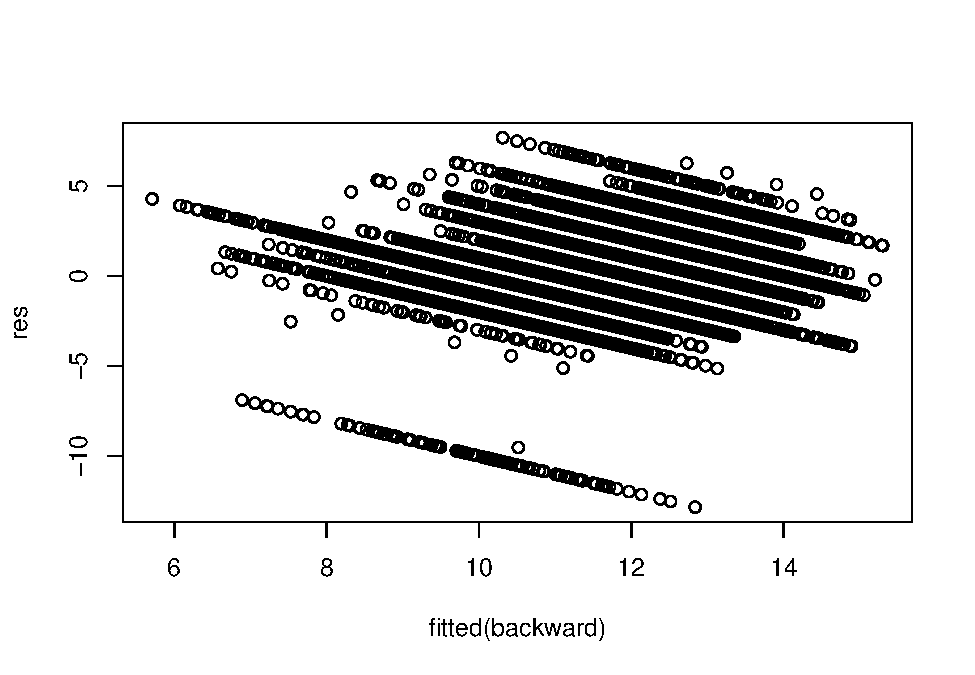
\includegraphics{pstat_126_project_Week1_files/figure-latex/unnamed-chunk-14-1.pdf}
Conclusion: As we can see, there are a few blocks that are heavily
correlated. For example, Mother and Father education are correlated, G,
G2, and G3 are all correlated as well as Weekend and Workday Drinking.
there are a few areas that seem to have nearly no correlation such as
freetime and Health. while there are a few that have a high negative
correlation such as weekend alcohol consumption and all the G variables.
High correlation indicates that variables are not independent from one
another, therefore, we will need to drop some of them before building
our model.

\end{document}
